\documentclass[12pt]{article}
\usepackage{amsmath}
\usepackage{graphicx}
\usepackage{hyperref}
\usepackage[latin1]{inputenc}
\usepackage{exercise}
\usepackage{cancel}
\usepackage[margin=2cm]{geometry}
\usepackage{float}
\usepackage{wrapfig}
\usepackage{amssymb}
\setlength\parindent{0pt}

\title{Neural Signal Analysis - Notes}
\author{Francesco Negri - Eleonora Borsani}
\date{A.Y. 2021-2022}

\begin{document}
\maketitle

\tableofcontents
\newpage

\section{Introduction}
\graphicspath{ {./images/1/} }
The application of a stimulus to the nervous system leads to changes determined by
two main properties:
\begin{itemize}
    \item \textbf{Excitability:} the capability of a nerve cell to react to an
    incoming impulse.
    \item \textbf{Plasticity:} certain permanent functional transformations arise in
    particular systems of neurons as a result of appropriate stimuli or their
    combination.
\end{itemize}
The communication between neurons occurs through action potentials, as shown in the
following picture.
\begin{figure}[H]
    \includegraphics[scale=0.35]{1_1}
    \centering
\end{figure}
Measuring, analyzing, and processing brain signals is done for several reasons, but
the three main ones are listed below:
\begin{itemize}
    \item \textbf{Learn} more about the brain functioning.
    \item \textbf{Mimic} the brain functions in an artificial way - i.e. neuromorphic
    engineering.
    \item \textbf{Employ} brain signals for control and communication, as in the
    case of prosthetics.
\end{itemize}
The nerual code can either be read or written by exploiting several distinct
techniques exhibiting different levels of:
\begin{align*}
    \begin{matrix}
        \textbf{Invasiveness} && \textbf{Risk} &&
        \textbf{Spatial resolution} && \textbf{Temporal resolution}
    \end{matrix}
\end{align*}
The technology nowadays allows fair degrees of spatial and temporal resolution, with
the main reading techniques being fMRI, PET, optical imaging, EEG, ECoG, MEA,
single neuron, and others. Notice that also the number of reading sites is constantly increasing, due to the
exploitation of multiple electrode devices.
\begin{figure}[H]
    \includegraphics[scale=0.375]{1_2}
    \centering
\end{figure}
The multi-scale brain model presented above aims at showing the different levels at
which the brain activity can be investigated, in terms of spatial, temporal,
and topological scales.
Let's stress once more that the brain can be studied at different level of complexity,
which are somehow related to the risk due to the techniques involved to do so.
\begin{figure}[H]
    \includegraphics[scale=0.35]{1_3}
    \centering
\end{figure}
Notice that in general the functional unit of the brain is not a single neuron.\\
Two main classes of techniques exist: the \textit{in vitro} and \textit{in vivo} ones. Generally, the
second family is more complex to employ, as it requires not to damage the brain of
the experiment subject. One of the principal technologies to study \textit{in vitro} networks
is MEAs (Micro Electrode Arrays), which are able to detect the activity
of the network at several recording sites and for extended time periods. An issue
related to MEAs is the difficulty often encountered in analysing the recorded data
and interpretating the results in a meaningful way.\\
In general, by recording neural signals at high frequencies and close to few
neurons a signal made of spikes, indicating the firing of a neuron, can be obtained,
while by recording at higher distances the local field potetial (LFP) is instead
obtained, consisting in the low frequency component and accounting for several
neurons as a sort of superposition of their effects.\\
It is common to find in vitro neural networks since they are extensively employed in
research due to their fair level of organization and to the capability to easily
record their activity with arrays of electrodes. Nonetheless, some issues related to
\textit{in vitro} networks are the fact that they have no fidelity w.r.t. \textit{in vivo} neurons,
starting from the fact that they generally arranged in 2D layers, instead of
more complex three-dimensional networks.
\begin{figure}[H]
    \includegraphics[scale=0.275]{1_4}
    \centering
\end{figure}
Another crucial concept is the one of brain modularity, as a matter of fact the brain
is redundant and intrinsically modular, due to the fact that it is composed of
local networks that are embedded into networks of networks.\\
Other wideley spread techniques are in vitro brain slices and \textit{in vivo} surgical
procedure. In both cases data are collected from biological tissue by means of
MEAs or similar technologies.\\
The analysis of neural signals is usually performed on spike trains, which are
derived by filtering the raw signal recorded from electrodes and by detecting the
spikes present in it. Notice that the crucial point is not the magnitude of a
certain spike, rather its position on the time axis, indicating when it was fired.
\begin{figure}[H]
    \includegraphics[scale=0.5]{1_5}
    \centering
\end{figure}
It is important to point out that the shape of a spike is highly influenced by the
position of the measuring electrode w.r.t. the neuron that emitted it, enabling
the researchers to recognize all the spikes emitted by the same source - i.e. a
particular neuron - and this is called spike sorting.\\
The main areas of research in this subject are reported in the following list:
\begin{itemize}
    \item Identification and classification of spike events (spike detection and
    spike sorting).
    \item Techniques for measuring the association between neural spike trains.
    \item Quantification of the neural response to a stimulus.
\end{itemize}
Finally, let's highlight that the high number of electrodes employed in today's
research implies a number of new challenges concerning data aquisition, storage,
and analysis.
\newpage

\section{Spike Detection}
\graphicspath{ {./images/2/} }
\subsection{Introduction}
Neural signals are firstly recorded as raw data. They exhibit two
main components:
\begin{itemize}
    \item Local field potentials (LFPs) exist at low frequencies (0.1-300 Hz).
    \begin{figure}[H]
        \includegraphics[scale=0.45]{2_1}
        \centering
    \end{figure}
    \item Spikes (MUA) exist at higher frequencies (300-3000 Hz).
    \begin{figure}[H]
        \includegraphics[scale=0.45]{2_2}
        \centering
    \end{figure}
\end{itemize}
The signal is obtained through extracellular recordings,
then amplified and filtered. There are 3 possible situations, according to the
distance of the electrode tip from the neurons:
\begin{itemize}
    \item \(<50\,\mu{m}\): the SNR is good enough to distinguish the activity
    of a single neuron (single unit).
    \item \(50\sim150\,\mu{m}\): spikes are still detected, but the difference in
    their shape is masked by the noise (multi-unit activity or MUA).
    \item \(>150\,\mu{m}\): spikes cannot be detected and they contribute to
    the noise.
\end{itemize}
\begin{figure}[H]
    \includegraphics[scale=0.35]{2_3}
    \centering
\end{figure}
\newpage
When recording data from 1 electrode, there are two patterns of activity:
\begin{itemize}
    \item Spike: single over-threshold signal representing the electrical
    activity of one or more neurons.
    \item Burst: sequence of highly packed spikes often occurring simultaneously
    on several channels and giving rise to a phenomenon known as
    'network burst'.
\end{itemize}
In the following it is show the Data Preprocessing workflow:
\begin{figure}[H]
    \includegraphics[scale=0.6]{2_4}
    \centering
\end{figure}
Spike trains are defined as the temporal sequence of spiking events, without
any regard of time. Spike trains are mathematically defined as follow:
\begin{itemize}
    \item Single channel spike train: \(ST(t)=\sum_{s=1}^{N}\delta{(t-t_s)}\)
    \item Multiple channel spike train: \(ST_j(t)=\sum_{s=1}^{N_j}\delta{t-t_s}\)
    with \(j=1,...,M\)
\end{itemize}
\begin{figure}[H]
    \includegraphics[scale=0.45]{2_5}
    \centering
\end{figure}
\textbf{Spike Detection:} it consists in recognizing the spikes within the raw data.\\
It is the most important step of the analysis, as it affects all
the subsequent steps.\\
\textbf{Spike Sorting:} associate each spike to a specific putative source
(classify spikes).\\
When performing Spike Detection there are two main issues:
\begin{itemize}
    \item Reliability (of the selected detection method)
    \item Precise position (of the detected peaks in the spike train)
\end{itemize}


\subsection{Spike Detection algorithms}
Therefore, several algorithms (each one with pros and cons) have been developed.
These spike detection algorithms can be divided into 3 families:
\begin{itemize}
    \item Thresholding: it is assumed that spikes peak-to-peak amplitude is larger
    than the noise level.
    \item Energy operator: non-linear energy operator accentuating high frequency
    contet, i.e. spikes.
    \item Template matching: it is an approach based on the spike shape,
    involving Spike Sorting.
\end{itemize}
\subsubsection{Thresholding algorithms}
\paragraph{Simple Hard Threshold}
A threshold value is defined (either positive or negative). If the signal
overcomes the threshold, then a spike is detected. A refractory period (RP)
is employed to account for subsequent samples overcoming the threshold after
a spike detection.
\paragraph{Hard Threshold} Notice this algorithm is applied also to
absolute-valued signals. It involves 2 distinct main steps:
\begin{itemize}
    \item Application of a threshold
    \item Spike identification
\end{itemize}
A time window denoted by \(T\) is applied to the signal, centering the window
\(\frac{1}{3}T\) before the detected spike. The length of \(T\) is to be
carefully chosen, usually \(1-3\,ms\), as it must minimize the likelihood that
more than one spike is captured in the window.\\
The threshold (\(Thr\)) is defined in several ways:
\begin{itemize}
    \item \(Thr=n\sigma[V]\): \(n\) times the standard deviation (SD) of
    the noise.
    \item \(Thr=aP2P[V]\): fraction of the full amplitude (peak-to-peak) of
    the signal.
    \item \(Thr=n\sigma_N[V]\): \(n\) times the SD estimated from the Median
    Absolute Deviation (\(MAD\)), with \(MAD=median(|x-median(x)|)\).
\end{itemize}
\paragraph{Hard Threshold Local Maxima}
This method is very similar to the previous ones, but the spike position is
associated to the local maxima (and not set at the time of the first sample
overcoming the threshold).
\paragraph{Hard Threshold Differential Threshold}
A sliding window \(W\) is sized to contain at least one spike and is shifted
over the signal. The peak-to-peak threshold \(k\sigma\) is a multiple of the
noise standard deviation. Then, a spike is detected in the \(i-\)th window
when \([(max_i-min_i)\ge{k\sigma}]\), with \(i=1,...,\frac{T}{W}\) and \(T\)
being the signal whole duration.\\
This approach exhibit a major issue: undersampling if more spikes are found in
a single window (typically at the window borders).
\paragraph{Precision Timing Spike Detection (PTSD)}
This method solves the undersampling issue. The max and min of each selected
window is selected. A refractory period RP is also considered. This technique
is more demanding from the computational point of view, but it allows to detect
also the spikes passing through the boundaries of the considered bin.
\subsubsection{Energy operator algorithms}
\paragraph{Signed Energy (SE)}
A moving window is used to scan the signal. For each time window the energy is
computed as follow:
\begin{align*}
    SE(i)=\frac{1}{W}\sum_{j=i-\frac{W}{2}}^{j+\frac{W}{2}}V(j)^2
\end{align*}
The result is multiplied by +1 when the average amplitude of the raw signal is
positive, -1 when negative.
\paragraph{Nonlinear Energy Operator (NEO)}
The NEO is defined such that:
\begin{itemize}
    \item Constant voltage or zero \(\Rightarrow NE=0\)
    \item Waveform rapidly varying and a large amplitude
    \(\Rightarrow NE \text{ is maximum}\).
\end{itemize}
The \(NE\) of a signal \(x(n)\) is defined as:
\begin{align*}
    \psi[x(n)]=x^2(n)-x(n+1)\cdot x(n-1)
\end{align*}
Notice that the NEO is defined for each sample \(i\) and computed within a
window \(W\) centered in \(i\).\\
As a consequence, the NEO is large only when the signal \(x(n)\) is high is both
power and frequency. This method works especially well as a spike is generally
characterized by localized high frequencies and an increase in instantaneous
energy.\\
The threshold is defined as a scaled mean of the NEO:
\begin{align*}
    Thr=C\frac{1}{N}\sum_{n=1}^{N}\psi[x(n)]
\end{align*}
\subsection{Performance evaluation}
In order to assess the performance of a Spike Detection algorithm, a groundtruth
is to be defined, such that several metrics of the tested algorithm can be
computed. A groundtruth is a collection of information (typically a dataset)
which is known to be true, opposed to information provided by inference.
There are 3 main types of groundtruths:
\begin{itemize}
    \item Experimental groundtruth: neurons are recorded into two distinct ways,
    extracellular and intra-cellular (or juxtacellular), then a researcher uses
    the precise intra-cellular recordings (exhbiting precise timing and
    localization) to find the same spikes into the extracellular signal.
    \item Computational groundtruth: data are synthetic and produced by a
    model reproducing the behaviour of a network of neurons under different
    conditions. In particular, this method enables the researcher to test the
    Spike Detection algorithms against dataset with different characteristics,
    such as different signal-to-noise ratios (SNR).
    \item Hybrid groundtruth: natural and synthetic data can be mixed as well. In
    particular, it is common to exploit manually detected and sorted spikes to be
    fed into computational models as input.
\end{itemize}
Several distinct metrics might be taken into account when evaluating the
performance of Spike Detection algorithm, in particular the most used ones are:
\begin{itemize}
    \item Error count:
    \begin{itemize}
        \item Type I error \(\Rightarrow\) False Positive (FP): incorrect
        inclusion of noise, or spikes or other cells.
        \item Type II error \(\Rightarrow\) False Negative (FN): omission of
        true spikes.
    \end{itemize}
    \item Evaluation of the position of the detected spike (mean error)
    \item ROC curve
\end{itemize}
Let's define the following variables:
\begin{itemize}
    \item \(NREF\): number of reference spikes (true spikes present in
    the groundtruth dataset)
    \item \(NDS\): number of detected spikes (spikes identified by the
    tested Spike Detection algorithm)
    \item \(NCS\): number of correspondent spikes (spikes correctly
    identified by the algorithm matching the groundtruth data)
\end{itemize}
At this point, the following expressions for False Positives and False Negatives
can be derived:
\begin{align*}
    \text{False Positives}\Rightarrow FP=NDS-NCS
    \quad\quad\quad
    \text{False Negatives}\Rightarrow FN=NREF-NCS
\end{align*}
\begin{figure}[H]
    \includegraphics[scale=0.4]{2_6}
    \centering
\end{figure}
Another way to rapidly visualize and assess the performance are the Receiver
Operating Characteristic (ROC) curve and the Area Under the Curve (AUC), reducing
the curve to a single scalar value between 0 and 1. Notice that the ROC curve
provides information regarding False Positives, but nothing is said about
False Negatives.\\
Let's also list the following metrics:
\begin{align*}
    \begin{matrix}
        TP_{rate} && \frac{TP}{P}\\
        FP_{rate} && \frac{FP}{N}=1-specificity\\
        Sensitivity && \frac{TP}{TP+FN}=\frac{TP}{P}=TP_{rate}\\
        Specificity && \frac{TN}{TN+FP}=\frac{TN}{N}\\
        Accuracy && \frac{TP+TN}{P+N}\\
        Performance && \frac{TP}{FP+FN}\\
        Efficiency && \frac{Performance}{Performance+1}
    \end{matrix}
\end{align*}
\newpage

\section{Spike Sorting}
\graphicspath{ {./images/3/} }
\subsection{Introduction}
Spike Sorting can be defined as the grouping of spikes into clusters
according to the similarity of their shapes.\\
This is useful only if the following assumption is made: each neuron tends
to fire spikes with a peculiar (distinguishable) extracellular shape.
As a consequence, it is possible to determine the activity of each one of these
neurons according to the measured spikes associated with it through Spike Sorting.\\
There are 3 reasons making Spike Sorting useful:
\begin{itemize}
    \item Increase the scale: as modern devices (MEAs) record from large populations
    of neurons at the same time, it is desirable to derive the inidividual
    activity of as many neurons as possible.
    \item Carry out new types of analysis: it might be interesting to study
    connectivity patterns of close-by neurons or perform analysis at
    single-neuron level.
    \item Have acess to sparsely firing neurons: it is desirable to understand
    the typical patterns of a specific kind of neuron, allowing to study its
    specific function.
\end{itemize}
Despite everything, Spike Sorting still present a number of major problems:
\begin{itemize}
    \item Dealing with background noise.
    \item Neurons in the same area might emit spikes with a similar shape (there
    is no way to perfectly know which neuron fired apart from imaging techniques).
    \item Neurons in the same area might emit spikes with a smaller amplitude.
    \item Background activity of distant neurons pollute the recorded signal.
    \item Waveform misalignment.
    \item Variation of the spike shape as a function of recent firing history
    (not time-invariant shape).
\end{itemize}
In the following an image of the whole Data Recording, Spike Detection, and
Spike Sorting process:
\begin{figure}[H]
    \includegraphics[scale=0.45]{3_1}
    \centering
\end{figure}


\subsection{Spike Sorting methods}
When it comes at Spike Sorting, there are 3 main approaches:
\begin{itemize}
    \item \textbf{Amplitude discriminator:} separate spikes according to their amplitude.
    This method does not take into account the shape of a spike, only its
    amplitude.
    \item \textbf{Template matching:} select a characteristic spike shape for each cluster
    and divide the spikes among the clusters via matching with the templates,
    according to an appropriate distance measure. The main issues of this
    approach is that the templates might need to adjust during the experiment
    and that it is necessary a good way to select the templates.
    \item \textbf{Window discriminator:} assign spikes crossing one or more windows
    to the same neurons. Also in this case issue may arise, especially spike
    shapes might overlap.
\end{itemize}
In general, Spike Sorting is carried out by following the steps shown below:
\begin{figure}[H]
    \includegraphics[scale=0.5]{3_2}
    \centering
\end{figure}
\subsubsection{Filtering}
The first step consists in filtering out the low frequency components
(\(<\) 300 Hz), in particular the local field potentials, in order to visualize
spikes.
To do so, a band 300-3000 Hz band-pass filter is employed: all the
frequencies outside the specified range are rejected.
\subsubsection{Spike Detection}
Spikes are commonly detect by using an amplitude threshold, as seen in the
previous chapter. The optimal threshold can be set manually or automatically
computed as a multiple of the standard deviation (SD) of the signal, where
\begin{align*}
    SD=\sigma=median\biggl(\frac{|x|}{0.6745}\biggr)
\end{align*}
\subsubsection{Feature Extraction}
Let's set the number of observations (i.e. spikes) to \(n\) and the
variables (data points) to \(m\), thus a \(m\)-dimensional space is obtained.
The idea is to extract a number of features \(p\), such that it has a lower
dimensionality (\(p<m\)).\\
The \(p\)-dimensional features can be selected in different ways:
\begin{itemize}
    \item Take basic properties of the spikes (amplitude, width, energy, ...),
    not optimal in differentiating spikes.
    \item Select a low number of components from a dimensionality reduction
    technique, such as PCA. Notice that these components represent the directions
    of maximum variance of the data, not necessarily the best separation.
    \item Use wavelets, obtaining a time-frequency decomposition of the signal
    with optimal resolution in both time and frequency domains.
\end{itemize}
\paragraph{Principal Component Analysis (PCA)}
It is an unsupervised dimensionality reduction technique, which can be used
also for feature extraction purposes. Data are rotated according to a new space
having the orthogonal axes in the directions of maximum variance, then the new
obtained principal components are ordered by their contribution to the overall
variance, allowing to select only a fraction of the total number of components,
still approximating the original data fairly well. Low variance is often
interpreted as noise.
\paragraph{Wavelets}
The wavelet transformation (WT) is a time-frequency representation of the signal,
similar to the Fourier transform, but breaking the signal into its wavelets.
It may be defined as the convolution between the signal \(x(t)\) and the
wavelet functions \(\psi_{a,b}(t)\):
\begin{align*}
    W_\psi X(a,b)=\left\langle x(t)|\psi_{a,b}(t) \right\rangle
    \quad\quad\quad\quad\text{with}\quad
    \psi_{a,b}(t)=|a|^{-\frac{1}{2}}\psi\biggl(\frac{t-b}{a}\biggr)
\end{align*}
where \(a\) and \(b\) are scale and translation parameters.\\
Contracted wavelet function matches the high-frequency components, while
dilated wavelet matches the low-frequency components, thus details of the signal
at several scales can be obtained.\\
The wavelet method coefficients are then selected such that they allow to
distinguish well the spike shapes, in particular multi-modal distributions
are preferred and unimodal distributions are to be avoided.
\subsubsection{Clustering}
The final step of spike sorting is to group spikes with similar features into 
clusters, corresponding to different neurons. Different approaches are available:
\begin{itemize}
    \item Manual clustering
    \item Bayesian classification
    \item Expectation-Maximization methods
    \item Hierarchical clustering
    \item K-Means
    \item Superparamagnetic clustering
\end{itemize}
\paragraph{Superparamagnetic Clustering}
This method is inspired by statistical mechanics, it does not assume
a-priori distributions for the data, and exploit only one parameter to
form clusters: temperature.\\
The \(p\)-selected features of a generic \(i\)-th spike are represented by a
point \(x_i\) in a \(p\)-dimensional phase space. Then, let's define the
interaction strength between two points \(x_i\) and \(x_j\):
\begin{align*}
    J_{ij}=
    \begin{cases}
        \begin{matrix}
            \frac{1}{K}\exp{\biggl(-\frac{\|x_i-x_j\|^2}{2a^2}\biggr)} && \text{if}\,x_i\,\text{is a nearest neighbor of}\,x_j \\
            0 && \text{else}
        \end{matrix}
    \end{cases}
\end{align*}
where \(a\) is the average nearest-neighbor distance and \(K\) is the
number of nearest neighbors.
As a consequence, similar spikes will exhibit a strong interaction.\\
At this point, a random state is assigned to each point \(x_i\) and \(N\) Monte
Carlo iterations are run for different temperatures \(T\). A point \(x_i\) is
randomly selected and its state is randomly changed to \(s_{new}\).
The probability that the nearest neighbors of \(x_i\) will change their state
to \(s_{new}\) is given by:
\begin{align*}
    p_{ij}=1-\exp{\biggl(-\frac{J_{ij}}{T}\delta_{s_i,s_j}\biggr)}
\end{align*}
This implies that close points will change their status together,
forming clusters of spikes with similar shape.\\
In particular
\begin{itemize}
    \item High temperatures correspond to a low probability of
    changing the state \(\Rightarrow\) states change randomly, thus no clusters
    are formed (paramagnetic phase).
    \item Low temperatures correspond to a high probability of changing to the
    same state, regardless of the interaction strength \(J_{ij}\)
    \(\Rightarrow\) all states are changed to the same, thus all spikes belong
    to the same cluster (ferromagnetic phase).
    \item Medium temperatures correspond to a phase in which only similar spikes
    will change their state together, forming meaningful clusters
    (Superparamagnetic phase).
\end{itemize}


\subsection{Miscellaneous}
In the following are reported some further remarks and considerations concerning
Spike Sorting.
\subsubsection{Spike Sorting issues}
The main issues when it comes to Spike Sorting are listed below:
\begin{itemize}
    \item \textbf{Electrode Drift:} waveforms of a given neuron vary over
    time and may be assigned to multiple clusters.
    \item \textbf{Tetrodes:} tetrode recordings can be exploited to improve
    spike sorting results, since they allow the visualization of single
    neurons from different positions.
    \item \textbf{Overlapping Spikes:} this phenomenon can be observed when
    two close-by neurons fire in synchrony or with a small delay. Still 
    an open issue in Spike Sorting.
    \item \textbf{Bursting Cells:} a burst is the firing of a fast sequence
    of spikes by a neuron. Successive spikes in a burst may have decreasing
    amplitude and may be mistakenly considered as separate clusters.
\end{itemize}
\subsubsection{KiloSort}
The aim is to develop a fully automated, scalable, and accurate spike sorter,
removing the burden of this task from researchers. It belongs to the template
matching class of Spike Sorting algorithms.
The main hypothesis of KiloSort is that spatial and temporal shapes of a waveform
provide all the information necessary to assign a given spike to a neuron.
This algorithm exploits template matching in both Spike Detection and Spike
Sorting, which are condensed into a single unified model describing the voltage
\(V\) of channel \(i\) at the time instant \(t\):
\begin{align*}
    V(i,t)=\sum_{k=1}^{N_{spike}}A_{\sigma(k)}(i,t-t_k)\cdot x(k) + noise
\end{align*}
with \(A_{\sigma(k)}(i,t-t_k)\) being the spike template for the \(k\)-th neuron
and \(x(k)\) the amplitude of the spike emitted by the \(k\)-th neuron.
\subsubsection{Performance evaluation}
Different Spike Sorting methods can be compared by testing them on simultaneous
extracellular and intra-cellular recordings datasets, in a similar fashion w.r.t.
Spike Detection. The same metrics are generally used. The SpikeForest project
aims at benchmarking and testing the finest and most recent Spike Sorting
algorithms.
\newpage

\section{Spike Analysis}
\graphicspath{ {./images/4/} }
\subsection{Introduction}
As already stated in the previous chapters, it is well-known that in general the electrophysiological
signal (acquired from a single electrode) is characterized by 2 distinct patterns:
\begin{itemize}
    \item \textbf{Spike:} a single over-threshold signal representing the activity of one or
    more neurons (typically a so-called unit or channel).
    \item \textbf{Burst:} a sequence of highly packed spikes often occurring simultaneously on
    several channels and giving rise to a phenomenon known as network burst.
\end{itemize}
\begin{figure}[H]
    \includegraphics[scale=0.4]{4_1}
    \centering
\end{figure}


\subsection{Data visualization tools}
The first preliminary steps of Spike Analysis consist in taking a look at the raw data, then
deriving the spike train for each channel and visualize it. Therefore, it might be useful to define
a set of proper plots and metrics for data visualization.
\subsubsection{Raw data multi-channel plot}
The following plot shows the activity - i.e. voltage - recorded by 8 distinct electrons as a
function of time.
\begin{figure}[H]
    \includegraphics[scale=0.4]{4_2}
    \centering
\end{figure}
\subsubsection{Raster Plot}
The Raster Plot (also known as Spike Raster) is done after Spike Sorting and it allows to visualize
at the same time the spike trains coming from multple recording electrodes on the same time axis.
It is common to observe consistent activation patterns across channels, as neurons influence each
other.
\begin{figure}[H]
    \includegraphics[scale=0.75]{4_3}
    \centering
\end{figure}
\subsubsection{Task-Related Raster Plot}
The Task-Related (or Stimulus-Related) Raster Plot is similar to the ordinary Raster Plot, even if it
has a quite different meaning: the multiple lines do not represent channels, but portions of the
recording coming from just one channel. The signal portions are divided according to the execution of
a task or the receiving of a stimulus.
\begin{figure}[H]
    \includegraphics[scale=0.4]{4_4}
    \centering
\end{figure}
\subsubsection{High-Density Data Raster Plot}
This is once again a type of Raster Plot. Data comes from several channels and they cover a relatively
large span of time. As a consequence, it is almost impossible to distinguish single spikes by eye,
thus this high-density plot is usually inspected by looking at the shaded regions, as they exhibit a
higher concentration of fired spikes, implying a greater activity.
\begin{figure}[H]
    \includegraphics[scale=0.6]{4_5}
    \centering
\end{figure}
\subsubsection{Spike Count and Firing Rate metrics}
\paragraph{Spike Count}
This metric is obtained by dividing the time axis into equal bins \(\Delta{t}=[t_a,t_b]\) and just
counting the number of spikes \(N_{ab}\) occurring in each bin.
Then, an histogram showing the Spike Count can be plotted.
\paragraph{Instantaneous Firing Rate}
By simply taking the Spike Count and dividing it by the bin size, the Instantaneous Firing Rate (IFR)
can be derived. 
\begin{align*}
    IFR=r(t)=\frac{N_{ab}(t)}{\Delta{t}}
\end{align*}
The IFR is measured in spikes per second.
\paragraph{Spike Density Function}
The Spike Density Function (SDF) is obtained by associating a proper distribution (typically Gaussian)
to each single spike, then the SDF is derived by summing up the various individual distributions.
\begin{figure}[H]
    \includegraphics[scale=0.6]{4_6}
    \centering
\end{figure}
\paragraph{Array-Wide Firing Rate}
The Array-Wide Firing Rate (AWFR), often called Average Firing Rate (AFR), it is a sort of
IFR by taking into account the whole network - i.e. all the recorded channles, not just a single one.
This metric is often employed in neuropharmacology, in order to assess the time of response of a drug.\\
By setting the number of channels - i.e. the number of electrodes - to \(M\), the AFR is defined as:
\begin{align*}
    AWFR=awfr(t)=mean(IFR)=\frac{1}{M}\sum_{j=1}^{M}r_{j}(t)
\end{align*}
\paragraph{Mean Firing Rate}
The Mean Firing Rate (MFR) represents a single numerical metric of the activity of neurons for the
entire network (\(M\) channels). It is expressed as
\begin{align*}
    MFR=\frac{1}{T}\sum_{j=1}^{M}N_j
\end{align*}
where \(T\) is the considered time window (somehow corresponding to the previously seen \(\Delta{t}\)),
while \(N_j\) is the number of spikes recorded in the \(T\) interval for the \(j\)-th electrode.\\
Notice once again that both IFR and AWFR are functions of time, continuous in the time-domain, while
MFR is a single value giving information on the average degree of activation of the whole neural
network in a determined time interval.\\
The following plot illustrates the Mean Firing Rate, indicating the average neural activity, at
different concentrations of a brain inhibitor drug.
\begin{figure}[H]
    \includegraphics[scale=0.35]{4_7}
    \centering
\end{figure}
\subsubsection{Inter Spike Interval}
\paragraph{Inter Spike Interval}
The Inter Spike Interval (ISI) is the interval between two consecutive spikes. It is used to compute
the Inter Spike Interval Histogram (ISIH), an index of the probability that a spike is fired
a certain time \(\tau\) after a reference spike.
Given \(N\) spikes, the ISIH metric is computed as shown below:
\begin{align*}
    ISIH(\tau)=\frac{1}{N-1}\sum_{s=1}^{N-1}\delta{(t_{s+1}-t_{s}-\tau)}
\end{align*}
An histogram as the following one is often employed to visualize the metric.
\begin{figure}[H]
    \includegraphics[scale=0.5]{4_8}
    \centering
\end{figure}
Notice that it is common to have a higher probability close to the reference spike, while it tends to
decrease as the Inter Spike Interval grows. If the spike train is made of packed spikes alternating
to empty intervals, then the histogram will display 2 distinct peaks: one for the high frequency
component and one for the low frequency component.
\paragraph{Joint Inter Spike Interval}
The Joint Inter Spike Interval (JISI) is derived from the ISI and it is useful to evaluate the
relationship between pre-ISI and post-ISI intervals, for any spike of the train.
The probability JISIH for \(N\) spikes is computed as:
\begin{align*}
    JISIH(\tau_{post},\tau_{pre})=\frac{1}{N-2}\sum_{s=2}^{N-1}\delta{(t_{s+1}-t_{s}-\tau_{post})}\ast \delta{(t_s-t_{s-1}-\tau_{pre})}
\end{align*}
In this case the plot becomes tridimensional, however it can be displayed in 2D by using
colormaps.
\begin{figure}[H]
    \includegraphics[scale=0.45]{4_9}
    \centering
\end{figure}
\paragraph{Cross Inter Spike Interval}
The Cross Inter Spike Interval (CISI) works in a fashion similar to JISI, but it analyzes the
dependance between spikes of two different trains. The probability CISIH is given by:
\begin{align*}
    CISIH(\tau_{post},\tau_{cross})=\frac{1}{N-2}\sum_{a=1}^{N_a-1}\delta{(t_{a+1}-t_{a}-\tau_{post})}\ast \delta{(t_a-t_b-\tau_{cross})}
\end{align*}
\begin{figure}[H]
    \includegraphics[scale=0.5]{4_10}
    \centering
\end{figure}
\newpage

\section{Burst Detection}
\graphicspath{ {./images/5/} }
\subsection{Introduction}
The term \textbf{burst} lacks a formal definition. However, it is generally employed to indicate a recording period during which the spiking frequency is especially high, alternating with periods exhibiting a low spiking frequency (quiescence periods).
\begin{figure}[H]
    \includegraphics[scale=1]{5_1}
    \centering
\end{figure}
Neural bursting plays a key role in communication between neurons, in particular
burst neurons are crucial in \textbf{motor pattern generation and synchronization}.
A burst doesn't necessarily come from a network of neurons, but it can come also from a single neuron. Even 2 spikes can define a burst, and in this case they are called a doublet, while 3 are a triplet and so on. However, typically, when networks of neurons are taken into account, higher numbers of spikes are considered.\\
Basically, all neurons can burst if pharmacologically stimulated, however
it is common to observe autonomous bursting activity, especially in the following
types of neurons:
\begin{itemize}
    \item \textbf{IB:} intrinsically bursting neurons, mostly pyramidal neurons in
          layer 5.
    \item \textbf{CH:} chattering neurons, pyramidal neurons in layers 2, 3, and 4.
    \item \textbf{Interneurons:} present in the cortex.
    \item \textbf{LTB:} low-threshold bursters, that fire high-frequency bursts in
          response to injected pulses of current. They are localized in the hippocampus.
    \item \textbf{HTB:} high-threshold bursters, that fire bursts only in response to
          strong long pulses of current. They are localized in the hippocampus.
\end{itemize}
Bursting is also a peculiar feature of in vitro 'isolated' networks (i.e. systems that have neither exterior input nor output).
An 'in vitro' burst appearing at the level of a single electrode consists of a fast sequence of spikes with a duration equal to the sum of the Inter Spike Intervals (ISIs).
In vitro, burst generation is associated to the contemporary activation of different units more than the presence of intrinsic bursting neurons (i.e. pacemakers) which drive the entire network.
\paragraph{Why do bursts naturally occur?}
There are several hypotheses aiming to explain the importance of bursting activity in
neural computation.
\begin{itemize}
    \item \textbf{Bursts are more reliable than single spikes} in evoking responses in
          postsynaptic cells: excitatory post-synaptic potentials (EPSP) from each spike in a burst add up and may result in a superthreshold EPSP.
    \item \textbf{Bursts overcome synaptic transmission failure}: it has been shown
          that a synaptic release is more likely to occur in response to a bombardment
          of spikes (instead of a single spike).
    \item \textbf{Bursts evoke long-term potentiation}, thus affecting synaptic
          plasticity in a much greater way than single spikes.
    \item \textbf{Bursts have a higher signal-to-noise ratio} than single spikes, as
          the generation of bursts requires a higher threshold.
    \item \textbf{Bursts encode different features} of sensory input than single
          spikes. For example, neurons in the electrosensory lateral-line lobe (ELL) of weakly electric fish fire network induced-bursts in response to communication signals and single spikes in response to prey signals (Doiron et al. 2003).
    \item \textbf{Bursts have more informational content} than single spikes, in
          particular when analyzed as unitary events. This information might be encoded
          into the burst duration or in the precise temporal structure of inter spike
          intervals within a burst.
\end{itemize}
To conclude, it can also be pointed out that some believe that bursts are all-or-none events, whereas single spikes may be noise.
\subsubsection{Burst Train}
For the features listed before, it can be stated that a burst is characterized by \textbf{small Inter Spike Intervals} and a \textbf{certain number of spikes}.
\begin{figure}[H]
    \includegraphics[scale=0.25]{5_2}
    \centering
\end{figure}
From a mathematical point of view, some properties can be extracted from a burst, such as:
\begin{itemize}
    \item \(t_b\): the starting time of the burst.
    \item \(T_b\): the burst duration.
    \item \(A_b\): the burst amplitude, related to the spike frequency within the burst.
\end{itemize}
A \textbf{single-channel burst train \(BT(t)\)}can be defined as follow:
\begin{align*}
    BT(t) = \sum_{b=1}^{NB}A_b*\prod\biggl(\frac{t-t_b-\frac{T_b}{2}}{T_b}\biggr)
\end{align*}
with \(NB\) being the number of detected bursts.
The amplitude \(A_b\) of the burst is computed as:
\begin{align*}
    A_b=\frac{1}{T_b}\int_{t_b}^{t_b+T_b}\sum_{s=1}^{N}\delta{(t-t_s)}\,dt=\frac{N_{T_b}}{T_b}
\end{align*}
where \(N_{T_b}\) is the number of spikes within the considered burst.\\
Notice that if the burst is defined in this way, it can be represented as a sequence of rectangles:
\begin{figure}[H]
    \includegraphics[scale=0.2]{5_3}
    \centering
\end{figure}
For the multi-channel case (\(M\) channels are considered), the burst train
expression can be easily modified:
\begin{align*}
    BT_{j}(t) = \sum_{b=1}^{NB_{j}}A_b*\prod\biggl(\frac{t-t_b-\frac{T_b}{2}}{T_b}\biggr)
    \quad\quad\text{with}\,j=1,...,M
\end{align*}
\subsubsection{Burst Event}
Another meaningful way to represent bursts is the \textbf{burst event train \(BE(t)\)}, which can be defined as a point process in which each event corresponds to the starting time of a burst. It is similar to a spike train, even if the meaning is different. 
A single-channel burst event train is defined as
\begin{align*}
    BE(t)=\sum_{b=1}^{NB}\delta(t-t_b)
\end{align*}
Hence, to find a burst event, the first spike of each burst (\(t_b\)) needs to be found.\\
In the case the channels are multiple \(M\), the definition can simply be extended:
\begin{align*}
    BE_{j}(t)=\sum_{b=1}^{NB_{j}}\delta(t-t_b)
    \quad\quad\text{with}\,j=1,...,M
\end{align*}


\subsection{Burst Detection Algorithms}
There are several algorithms to identify bursts.
\subsubsection{String Method} 
This algorithm is based on some hypotheses:
\begin{enumerate}
    \item \textbf{A burst is characterized by a certain number of spikes} \(\rightarrow\) the minimum number of spikes belonging to a burst needs to be defined.
    \item \textbf{Spikes in a burst are very close} \(\rightarrow\) a maximum ISI value has to be set, to consider a spike as a part of a or not.
    \item \textbf{Bursts are far away at least hundreds of ms} \(\rightarrow\) a minIBI has to be set, to consider 2 bursts as separated or not.
\end{enumerate}
Typically, the following values are selected:
\begin{itemize}
    \item \(ISI_{max}=100\,ms\)
    \item Minimum number of intra-burst spikes \(=5\)
    \item For simplicity, \(IBI_{min}=ISI_{max}\)
\end{itemize}
Because this method has a minimal computation time, it allows the implementation of burst analysis in real-time, including statistical changes in burst variables, histograms of burst types, and patterns in combinations of burst variables.
\subsubsection{Wagenaar (WA)} 
The method developed in 2005 by D. A. Wagenaar tries to solve a problem caused by the fact that usually bursts are characterized by two main trends:
at the beginning (\textbf{burst core}) the spiking frequency is particularly high, while
it tends to become increasingly low as time passes (\textbf{burst tail}). In order to
better detect the bursts accounting for the differences of the two portions just described, a system considering two distinct ISI thresholds is employed. \\
The steps carried out by the algorithm are:
\begin{enumerate}
    \item Set the mean firing rate \(f\). If the signal is multi-channel, set \(f_j\) for the \(j\)-th channel.
    \item Define a maximum core ISI. Often the following values are used: \(th_{core}=1/4f\) or \(th_{core}=100\,ms\). The factor 4 ensures that only spikes that succeed each other faster than 4 times the average firing rate can be considered as part of the channel burst.
    \item Look for sequences having at least a minimum number of intra-burst spikes.
    \item Change the maximum ISI threshold to higher values, such as \(th_{tail}=1/3f\) or \(th_{tail}=200\,ms\).
    \item Keep looking for spikes before and after the burst core satisfying the
          new threshold condition.
\end{enumerate}
\subsubsection{Cocatre-Zilgien and Delcomyn (CZ)} 
It represents the first method based on the analysis of the ISI histogram, as it is highly informative about the spiking pattern of a specific recording channel, as shown in the picture below. In particular, it analyzes the histogram to detect the \textbf{critical interval value} in the distribution that represents the break between short intervals within a burst and longer intervals between bursts. When such a value is found, it is used as the 'threshold' to determine those intervals in the spike train that lie within a burst and those that lie between bursts and, thereby, to identify the beginning and end of each burst in the train. So, bursting activity tends to result in valleys.
\begin{figure}[H]
    \includegraphics[scale=0.32]{5_5}
    \centering
\end{figure}

\subsubsection{Selinger (SE)} 
This method exploits the ISI histogram (in a logarithmic scale) to derive the optimal ISI threshold, then it works as a standard single threshold algorithm. This technique tries to improve the identification of the spikes in the tail portion of a burst.
\begin{figure}[H]
    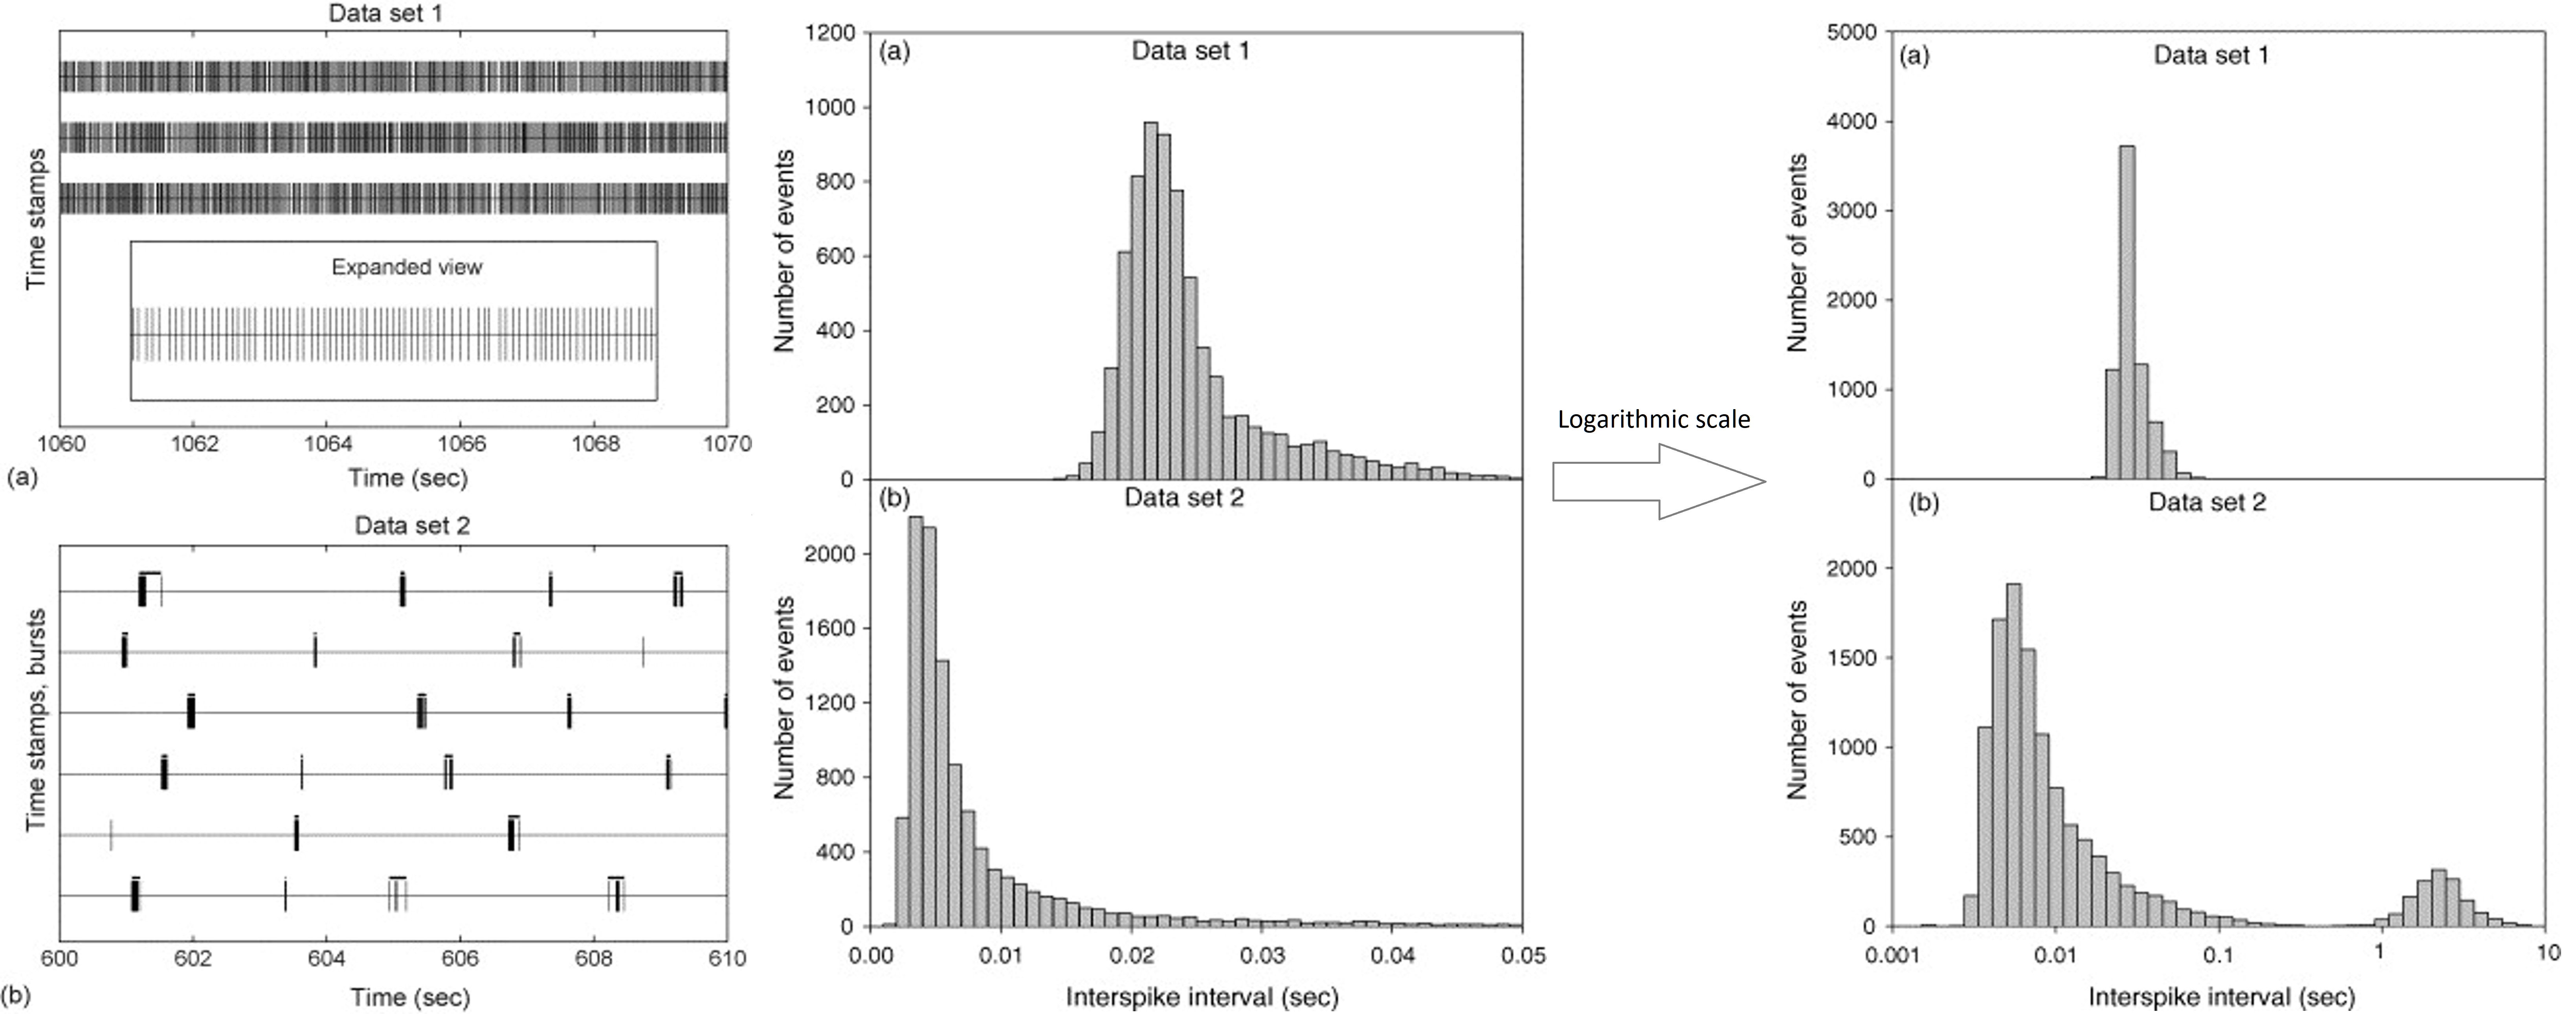
\includegraphics[scale=0.5]{5_6}
    \centering
\end{figure}

\subsubsection{Modified Selinger (SE-MOD)} 
It is a modified version of the Selinger method, consisting in a mix of the already presented techniques. It allows a better identification of the spikes at the boundaries of a burst event.
\begin{figure}[H]
    \includegraphics[scale=0.25]{5_7}
    \centering
\end{figure}
The asterisks in black represent the peaks and the one in red is the best point to separate the spikes (ISIth). If there is a burst, the approximation with the rectangular function is good from a mathematical point of view but, in reality, there are also some spikes with a lower frequency that yet belong to the burst.\\
With the string method, it's not always possible to detect all the spikes that belong to the burst. This because just a single threshold is used. Hence, it's better to define two of them: the \textbf{core} and the \textbf{tail thresholds}. The first is shorter, around \(100\,ms\), while the second is longer, between \(100\,ms\) and the ISIth. Obviously, this latter condition exists only if the ISIth is higher than \(100\,ms\). 
\begin{figure}[H]
    \includegraphics[scale=0.35]{5_8}
    \centering
\end{figure}
These images show recordings from in vitro culture, in particular the spontaneous activity (basal) and the activity
of an antagonist. In this second case there is a very long bursting activity.\\
It can be observed that from the basal to the antagonist activity there is a shift of the threshold. Moreover, notice that there are 2 peaks in the ISIh, that represent the two activities that can be observed in the bursts, where there is an area where the spikes are one near the other and another area in which they are more distant. The logISI algorithm is able to detect both cases. 

\subsection{Comparison of Algorithms}
Generally, it can be stated that all the implemented burst detection techniques proposed so far presents pros and cons, thus there is not an algorithm clearly prevailing on the others: different techniques perform better in different situations, according to the type of data that are intended to be analyzed.
\begin{figure}[H]
    \includegraphics[scale=0.3]{5_9}
    \centering
\end{figure}
In the previous image, a quantitative comparison among the algorithms is realized:
\begin{itemize}
    \item the asterisk compares statistical differences in the same group.
    \item the empty circle compares the results of a specific method in different experimental conditions.
\end{itemize}
What can be deduced is that:
\begin{itemize}
    \item The logISI (newBD) algorithm is able to reveal the strong increase of burst duration caused by BIC stimulation, as the SE algorithm, whereas WA and CH fail.
    \item At the same time, in the basal condition of APV experiment, the logISI detects the 'correct' number of bursts (as WA and CH), whereas the SE algorithm fails.
    \item Finally, the GE algorithm provides clearly wrong burst detection when applied to in vitro recordings of neuronal cultures.
\end{itemize}
\newpage

\end{document}